\documentclass[11pt,a4paper]{article}
\usepackage[margin=2.2cm]{geometry}
\usepackage[T1]{fontenc}
\usepackage[utf8]{inputenc}
\usepackage{lmodern}
\usepackage{microtype}
\usepackage{amsmath,amssymb}
\usepackage{booktabs}
\usepackage{graphicx}
\usepackage{xcolor}
\usepackage{caption}
\usepackage{subcaption}
\usepackage{enumitem}
\usepackage[colorlinks=true,linkcolor=blue!55!black,urlcolor=blue!55!black,citecolor=blue!55!black]{hyperref}
\captionsetup{font=small,labelfont=bf,width=0.95\textwidth}
\setlist{nosep,leftmargin=*}
\graphicspath{{../figures/}}
\newcommand{\Mz}{M0}\newcommand{\Mo}{M1}\newcommand{\Mt}{M2}
\definecolor{claimbg}{RGB}{245,247,250}
\newsavebox{\claimsavebox}
\newenvironment{claimbox}[1]{\par\medskip\noindent\begin{lrbox}{\claimsavebox}\begin{minipage}{\dimexpr\linewidth-2\fboxsep-2\fboxrule\relax}\setlength{\parskip}{2pt}\textbf{#1}\par\smallskip}{\end{minipage}\end{lrbox}\setlength{\fboxsep}{6pt}\setlength{\fboxrule}{0.5pt}\fcolorbox{black!45}{claimbg}{\usebox{\claimsavebox}}\par\medskip}

\title{\textbf{Does Internal Geometry Break Before Robot Behavior Does?}\\[4pt]
\large A preregistered test on SmolVLA/LIBERO: internal activations replace privileged simulator state for failure prediction but do not beat it, and the decodable orientation direction is not causally used}
\author{Fynn van Rießen\\[2pt]\small Repository: \href{https://github.com/jimfable/mech-int-vla}{github.com/jimfable/mech-int-vla} \quad Report commit: see Appendix~\ref{app:repro}}
\date{17 September 2026}

\begin{document}
\maketitle

%======================================================================
\section*{Executive summary}
\addcontentsline{toc}{section}{Executive summary}

\textbf{Question.} A robot policy sometimes fails. Do its \emph{internal activations} tell you that a failure is coming, beyond what you could already know from its \emph{outputs} and from \emph{privileged simulator state}? If yes, mechanistic interpretability buys something on vision-language-action (VLA) models. If no, it does not---at least not in this form.

\textbf{What we did.} We froze one public policy (SmolVLA fine-tuned on LIBERO), one manipulation task (``pick up the book and place it in the back compartment of the caddy''), and three nested failure predictors: \Mz{} (policy outputs only), \Mo{} (\Mz{} + privileged simulator state), \Mt{} (\Mo{} + internal signals built from a probe for the book's relative orientation). Every threshold, metric, and analysis step was preregistered and hash-locked before the held-out \emph{Locked Test} split (160 episodes, 8 perturbation conditions) was collected. The evaluator ran exactly once. Cost: 21.7 GPU-hours on one RTX~5090.

\textbf{Results (Figure~\ref{fig:headline}).}
\begin{enumerate}
\item \textbf{The preregistered primary claim fails, and fails cleanly.} \Mt{} beats \Mo{} in paired log loss by $+0.47\%$ (90\% cluster-bootstrap CI $[-1.2\%,\,+2.1\%]$; bar: $\geq 3\%$). The interval excludes the bar, but only by 0.9 percentage points: a 3\% lift is unlikely, a 1--2\% lift is not ruled out.
\item \textbf{Internals \emph{substitute} for privileged state.} \Mt{} beats the output-only baseline \Mz{} by $18.8\%$ in log loss ($\Delta$ log loss $-0.120$, CI $[-0.187,\,-0.052]$, both ends favourable); AUROC $0.667 \to 0.835$. A model that never sees the simulator state does as well as one that does.
\item \textbf{The decodable orientation direction is a readout, not a lever.} Patching the probe's 2-D subspace at the selected layer ($\alpha{=}0.25$; also $0.5$, $1.0$) moves the policy's action \emph{less} than a random direction of the same norm (median off-target ratio $4.0$; bar $\leq 0.25$), with the predicted sign in $48\%$ of 52 valid pairs (CI $[36\%,62\%]$; bar: CI above $50\%$). All 16 preregistered dose$\times$condition sensitivity cells fail specificity.
\item \textbf{No earlier alarm.} At a fixed 10\% episode-level false-positive rate, \Mt{} and \Mo{} detect 98\% of the 60 failures with identical median lead time (paired difference $0$ steps, CI $[0,0]$).
\end{enumerate}

\textbf{Takeaway.} On this policy and task, everything the internal orientation signal knows about upcoming failure is already in the privileged state, and the direction we can decode is not one the policy acts through. Per the preregistered decision table this is the ``neither lift nor specificity'' row: publish the negative result, stop the line.

\textbf{Confidence.} High that the measured numbers are what this protocol produces (single frozen run; every input content-addressed). Moderate that the conclusion generalises: one policy, one task, one layer, 158 valid episodes. Section~\ref{sec:limits} lists what would change our mind, with rough probabilities.

\begin{figure}[htbp]
\centering
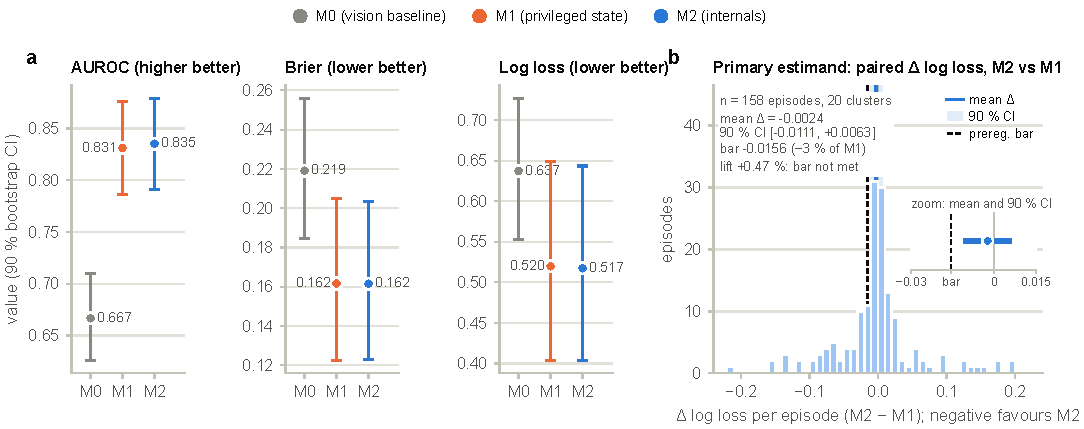
\includegraphics[width=\textwidth]{fig_headline.pdf}
\caption{\textbf{Headline result on the Locked Test (158 valid episodes, 20 init-state clusters).} \textbf{(a)} Failure-prediction quality per model with 90\% cluster-bootstrap intervals (10\,000 replicates, seed 260803). \Mo{} and \Mt{} are indistinguishable; both clearly beat \Mz{}. \textbf{(b)} The primary estimand: per-episode paired difference in log loss, $\ell^{\Mt}_e - \ell^{\Mo}_e$ (negative = \Mt{} better). Mean $-0.0024$, 90\% CI $[-0.0111, +0.0063]$; the preregistered bar of a 3\% relative improvement corresponds to $-0.0156$ (dashed) and lies outside the interval. 54\% of episodes lie within $\pm 0.02$. Lower is better for log loss and Brier; higher for AUROC.}
\label{fig:headline}
\end{figure}

\tableofcontents

%======================================================================
\section{Why this question}
\label{sec:why}
Interpretability on VLA models has produced decodable representations and steering demonstrations, but rarely a controlled test of whether reading the internals adds \emph{predictive} value over cheaper, non-internal diagnostics. That is the practical bar: a safety monitor built on activations must beat one built on the policy's own outputs and, ideally, one built on privileged information nobody has at deployment.

We designed the test as a nested comparison so that a positive result would be unambiguous and a negative result would still be informative. The ``boring'' alternatives were built in as baselines rather than tested afterwards:
\begin{itemize}
\item If internals only beat outputs (\Mt{} $>$ \Mz{}, \Mt{} $\approx$ \Mo{}), they \emph{substitute} for state you would otherwise need a simulator for---useful, but not new information.
\item If internals beat privileged state (\Mt{} $>$ \Mo{}), they carry information about the policy's own competence that the world state does not.
\item If a probed direction is causally used, moving it should move actions more than random directions of the same size do, and in the predicted direction.
\end{itemize}
Before touching the GPU we wrote down (\texttt{start.md}, \texttt{PREREG.md}) the estimands, the bars, the split logic, and a decision table mapping every outcome to a consequence. Our own toy-model evidence predicted the outcome we then observed: \Mt{} $\approx$ \Mo{} $\gg$ \Mz{} (Appendix~\ref{app:prereg}).

%======================================================================
\section{Claims}
\label{sec:claims}
All four claims below were preregistered as tests; the tiers are ours.
\begin{claimbox}{Claim 1 (systematic, preregistered primary): internal signals do not improve failure prediction over privileged state.}
Paired log-loss lift \Mt{} vs \Mo{} $= +0.47\%$, 90\% CI $[-1.2\%, +2.1\%]$ ($\Delta$ log loss $-0.0024$, CI $[-0.0111, +0.0063]$), bar $\geq 3\%$. \textbf{Fails.} Evidence: Section~\ref{sec:claim1}.
\end{claimbox}
\begin{claimbox}{Claim 2 (systematic, preregistered secondary): internal signals substitute for privileged state.}
\Mt{} vs \Mz{}: $\Delta$ log loss $-0.120$, CI $[-0.187, -0.052]$; relative lift $18.8\%$. \textbf{Holds.} Section~\ref{sec:claim1}.
\end{claimbox}
\begin{claimbox}{Claim 3 (hedged, preregistered): the probe subspace is not a causal lever at the tested layer and doses.}
Sign-correct $48\%$ [36\%, 62\%]; off-target ratio $4.03$ (bar $\leq 0.25$); 60\% of patched states leave the natural activation manifold. \textbf{Specificity fails at $\alpha \in \{0.25, 0.5, 1.0\}$.} The stronger multi-layer criterion could not be evaluated (Section~\ref{sec:claim3}).
\end{claimbox}
\begin{claimbox}{Claim 4 (narrow, preregistered): no lead-time gain.}
Median paired lead-time difference \Mt{} $-$ \Mo{} $= 0$ steps, CI $[0,0]$, bar $\geq 5$. \textbf{Fails.} Section~\ref{sec:claim4}.
\end{claimbox}

%======================================================================
\section{Setup}
\label{sec:setup}
\paragraph{Policy and task.} \texttt{lerobot/smolvla\_libero} (revision \texttt{31d453f7}), a SmolVLA policy with a SmolVLM2-500M backbone and a flow-matching action expert (10 denoising steps, 50-step action chunks, one executed action per step). Simulator: LIBERO-10 task~5, ``pick up the book and place it in the back compartment of the caddy''; primary object \texttt{black\_book}, planar symmetry order 2. Two 360$\times$360 cameras (agent view, wrist), 8-D proprioceptive state, 7-D relative actions.

\paragraph{Episodes and failure.} Closed loop, replanning every step, horizon 520 control steps after 10 settle steps. Success is LIBERO's own \texttt{check\_success}; failure is no success by step 520. A deterministic, frozen annotator assigns each failed episode a failure \emph{onset} step (missed grasp, dropped object, irrecoverable workspace exit, or terminal horizon), used only for lead time.

\paragraph{Perturbation conditions.} Eight cells of 20 episodes each, one per initial state: unperturbed (iid); the book rotated by $-37.5^\circ, -22.5^\circ, +22.5^\circ, +37.5^\circ$; the book displaced 4.5\,cm diagonally; the agent camera yawed $\pm 5^\circ$ with a 2\,cm lateral shift. The Calibration split used different rotation angles ($\pm 15/30/45^\circ$) and a 3\,cm axis displacement, so Locked Test conditions are held-out perturbations, not just held-out seeds.

\paragraph{Splits.} Fifty fixed initial states: 0--9 Discovery (stack reproduction, reality gate), 10--29 Calibration (all fitting and selection), 30--49 Locked Test. Reset seeds are derived from split, init, and cell; nothing crosses splits. Uncertainty is always a cluster bootstrap over the 20 init-state clusters (10\,000 replicates, 90\% percentile intervals, seed 260803), never over frames.

\paragraph{The three predictors.} All three are histogram-gradient-boosting classifiers (learning rate 0.03, 200 trees, 7 leaves, min 20 per leaf; family and hyper-parameters chosen on Calibration by grouped out-of-fold \Mo{} log loss, then frozen), predicting $p(\text{episode fails} \mid \text{state at step } t)$ at $t \in \{0,50,100,150,200\}$; every episode has total sample weight one.
\begin{itemize}
\item \textbf{\Mz{} (outputs only, 13 features):} how much the action chunk changes under counterfactual inputs (brightness $\times 0.85/1.15$, camera yaw $\pm 3^\circ$, object yaw $\pm 15^\circ$, planar shifts), spread of actions across 8 flow-noise draws, chunk norm and roughness.
\item \textbf{\Mo{} (+ privileged state):} relative end-effector/object/goal poses, symmetry-aware yaw, gripper opening, contact flags, task phase, plus \emph{coverage} features---distance to the nearest successful Calibration states in the same phase and the failure fraction among the 25 nearest.
\item \textbf{\Mt{} (+ internals, 8 features):} how the orientation probe's readout behaves under the same counterfactuals (equivariance error under object rotation, dispersion under brightness/camera/noise), the readout's norm and robust $z$-score against successful Calibration states, and a controllability gain and on/off-target ratio from minimum-norm interventions in the probe subspace. No \Mt{} feature uses simulator ground truth.
\end{itemize}

\paragraph{The probe.} Target: $[\cos 2\theta_{\mathrm{rel}}, \sin 2\theta_{\mathrm{rel}}]$ with $\theta_{\mathrm{rel}}$ the end-effector-to-book yaw (order-2 symmetry). Five preregistered candidate locations (VLM residual at layer 12; action-expert residual after layers 3 and 11, at flow steps $t{=}1.0$ and $0.5$). Selection rule: episode-weighted ridge regression, grouped 5-fold by init, circular MAE, lowest mean then preregistered preference within one SE. Selected: \texttt{early\_expert\_t1\_0} (width 720, mean over the 50 action tokens), MAE $0.253$\,rad vs. $0.332$ for a constant predictor and $0.315$ for proprioception alone. The probe is real but modest: it tracks about 15\% of a $15^\circ$ object rotation (median error $12.8^\circ$) on Calibration.

\paragraph{Causal test.} For a recipient state $h_r$ and a donor $h_d$ from a matched state (same phase and contact, gripper within 1\,cm, positions within 2\,cm, book orientation $30$--$90^\circ$ apart) we patch $h_r' = h_r + \alpha P (h_d - h_r)$ with $P$ the rank-2 projector onto the probe subspace, applied to all 50 action tokens at the selected layer and flow step, then read the policy's first action. Controls per pair: (i) a matched donor whose orientation differs by $<5^\circ$ (should do nothing), (ii) 1\,000 random rank-2 subspaces with the same shift norm, (iii) an off-manifold check---the patched state's mean distance to its 5 nearest natural Calibration activations must stay below the natural 95th percentile (3.89). Sixty pairs (3 outcome-blind seeds $\times$ 20), $\alpha$ frozen at $0.25$ on Calibration (smallest of $\{0.25,0.5,1\}$ meeting the off-manifold cap), $\alpha \in \{0.5, 1.0\}$ as sensitivity.

\begin{figure}[htbp]
\centering
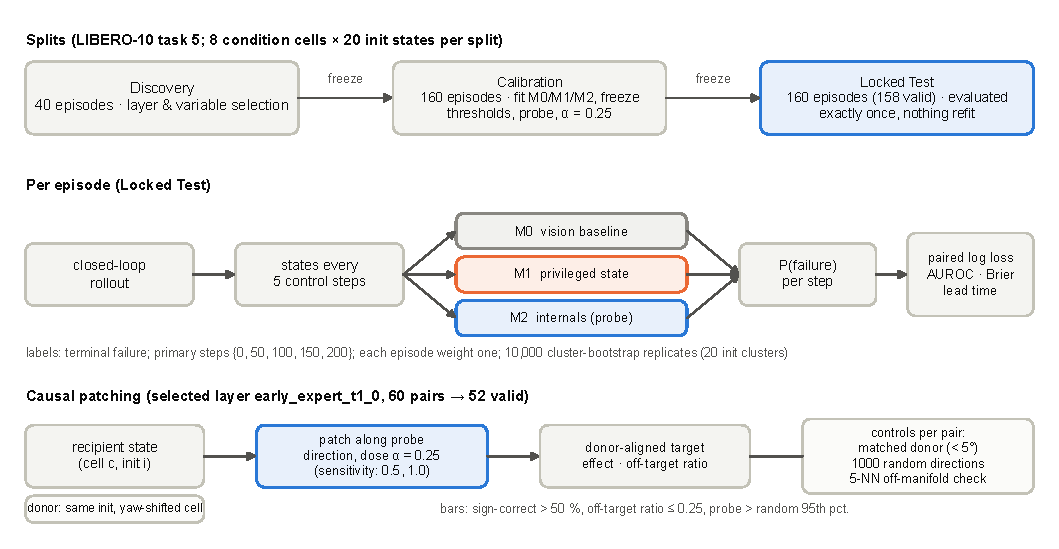
\includegraphics[width=\textwidth]{fig_pipeline.pdf}
\caption{\textbf{Study design.} Three strictly separated splits of 20 initial states each; all fitting, selection and threshold freezing happens on Calibration; the Locked Test is collected only after the freeze and evaluated once. Per episode: closed-loop rollout $\to$ states every 5 control steps $\to$ \Mz{}/\Mo{}/\Mt{} features $\to$ failure probability per step $\to$ paired log loss, AUROC, Brier, lead time. Bottom row: the causal test with its three controls.}
\label{fig:pipeline}
\end{figure}

\paragraph{Blinding and single evaluation.} Locked Test labels were never read by a human or by any fitting code before the evaluator ran; the run was monitored by counts and hashes only. Two loader defects (a trailing newline in a frozen lock file; a read-only mapping type) aborted the evaluator at input validation before any metric existed; each was fixed, tested, and recorded as an amendment before the rerun (Appendix~\ref{app:deviations}).

%======================================================================
\section{Claims 1 and 2: internals substitute for privileged state, and stop there}
\label{sec:claim1}
\paragraph{Why this experiment.} The primary comparison isolates the incremental value of internals over \emph{everything} non-internal; the secondary isolates their value over what a deployed monitor could actually see. The four possible outcomes were mapped to consequences in advance (Appendix~\ref{app:prereg}).

\paragraph{Result.} Table~\ref{tab:models} and Figure~\ref{fig:headline}. \Mo{} and \Mt{} are equivalent on every metric; both dominate \Mz{}. The primary interval on the relative lift, $[-1.2\%, +2.1\%]$, excludes the 3\% bar; its favourable end is 0.9 percentage points short of it. The \Mt{} vs \Mz{} interval excludes zero on the favourable side.

\begin{table}[htbp]
\centering\small
\caption{Locked Test failure prediction, 158 valid episodes. 90\% cluster-bootstrap intervals in brackets. Log loss and Brier: lower is better.}
\label{tab:models}
\begin{tabular}{lccc}
\toprule
& AUROC & Brier & Log loss \\
\midrule
\Mz{} outputs only & 0.667 [0.626, 0.710] & 0.219 [0.185, 0.256] & 0.637 [0.553, 0.727] \\
\Mo{} + privileged state & 0.831 [0.786, 0.876] & 0.162 [0.123, 0.205] & 0.520 [0.404, 0.649] \\
\Mt{} + internals & 0.835 [0.791, 0.879] & 0.162 [0.123, 0.204] & 0.517 [0.404, 0.643] \\
\midrule
\Mt{} $-$ \Mo{} (paired) & & & $-0.0024$ [$-0.0111$, $+0.0063$] \\
\Mt{} $-$ \Mz{} (paired) & & & $-0.120$ [$-0.187$, $-0.052$] \\
\bottomrule
\end{tabular}
\end{table}

\paragraph{Per condition.} Figure~\ref{fig:cells}. The \Mo{}/\Mt{} tie holds in all eight cells. Both are strongest where the perturbation is the probed variable (book yaw $+22.5^\circ/+37.5^\circ$: AUROC 0.93--0.98) and weakest in the iid and camera-yaw cells (0.66--0.73), where failures are rarer and less geometric. \Mz{} is near chance in the iid and camera $+5^\circ$ cells.

\begin{figure}[htbp]
\centering
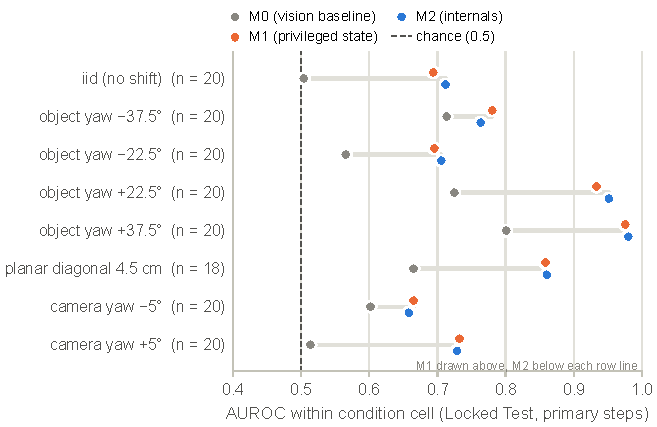
\includegraphics[width=0.92\textwidth]{fig_cells.pdf}
\caption{\textbf{AUROC per perturbation cell (20 episodes each).} Dotted line: chance. \Mo{} (orange) and \Mt{} (blue) coincide in every cell; the gap to \Mz{} (grey) is largest under book rotation, the variable the probe encodes.}
\label{fig:cells}
\end{figure}

\paragraph{Boring explanations we checked.}
\begin{itemize}
\item \emph{Overfitting on Calibration would hide a real gap.} It does not: the Calibration $\to$ Locked Test drop is similar for \Mo{} and \Mt{} (AUROC $0.937 \to 0.831$ and $0.938 \to 0.835$; Figure~\ref{fig:gap}), and their Calibration out-of-fold lift was already only $0.40\%$.
\item \emph{Underpowered.} The bar was set at a 3\% relative lift; the observed 90\% interval has half-width $1.7\%$ and its upper end is $2.1\%$. A true 3\% effect would most likely have shown, but a 1--2\% effect is compatible with the data; the preregistered bar, not the point estimate, is what fails.
\item \emph{The internal features are broken.} The probe they are built on beats every control on Calibration (circular MAE 0.253\,rad vs.\ 0.332 constant, 0.315 proprioception-only, 0.406 shuffled labels), and removing the \Mo{} coverage features raises the Calibration lift of \Mt{} over \Mo{} from 0.40\% to 1.20\%---still below the bar (Appendix~\ref{app:calib}). The features carry orientation information; it is simply redundant with the state block.
\item \emph{Kill switch.} A preregistered kill switch (any non-internal model with AUROC $\geq 0.95$ on Calibration would make the task too easy) did not trigger.
\end{itemize}

\begin{figure}[htbp]
\centering
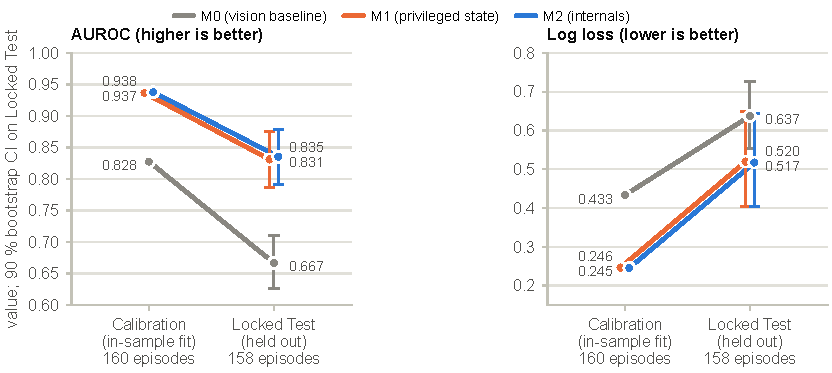
\includegraphics[width=0.85\textwidth]{fig_calibration_vs_locked.pdf}
\caption{\textbf{Generalisation gap.} AUROC and log loss on Calibration (out-of-fold, where all selection happened) versus the held-out Locked Test with new perturbation angles. All three models lose accuracy; the ordering and the \Mo{}/\Mt{} tie are unchanged.}
\label{fig:gap}
\end{figure}

\paragraph{Interpretation.} On this task the failure-relevant information carried by the orientation probe is a subset of what relative pose and coverage features already encode. That is exactly the ``substitute, not exceed'' row of the decision table. Note what it does \emph{not} say: it does not say internals are useless at deployment---\Mt{} needs no simulator and beats the output-only monitor by a wide margin.

%======================================================================
\section{Claim 3: the decodable direction is a readout, not a lever}
\label{sec:claim3}
\paragraph{Why this experiment.} A linear probe finding a variable proves decodability, not use. The patching test asks whether \emph{this} 2-D direction is one the policy's action expert reads from. Possible outcomes: specific and sign-correct (mechanism), sign-correct but unspecific (the direction overlaps something used but is not the used coordinate), or neither (readout only).

\paragraph{Result.} Figure~\ref{fig:causal}, Table~\ref{tab:causal}. Of 60 attempted pairs, 52 were valid (eight lacked an eligible donor or matched control; $\geq 30$ needed). The patch is small in absolute terms (median donor-aligned effect $-1.5\times 10^{-4}$ in standardised action units) and, crucially, \emph{smaller than random}: the 95th percentile of the 1\,000 norm-matched random subspaces is $1.0\times 10^{-4}$, giving a median off-target ratio of $4.03$ against a bar of $0.25$. The sign of the action change matched the donor's orientation in $25/52$ pairs ($48\%$, CI $[36\%, 62\%]$), the matched-donor control---which should be inert---moved the action in the ``predicted'' direction $54\%$ of the time, and only one of three seeds was positive. Sixty percent of patched states fell outside the natural activation manifold ($5$-NN distance above the Calibration 95th percentile), so the small effects are not explained by an overly cautious dose.

\begin{table}[htbp]
\centering\small
\caption{Selected-layer causal patching, $\alpha = 0.25$, 52 valid pairs.}
\label{tab:causal}
\begin{tabular}{lcc}
\toprule
Criterion & Bar & Measured \\
\midrule
Sign-correct rate (90\% CI) & CI above 50\% & 48.1\% [35.6\%, 62.2\%] \\
Median off-target ratio & $\leq 0.25$ & 4.03 \\
Target effect vs random p95 & target $>$ p95 & $-1.5\times10^{-4}$ vs $1.0\times10^{-4}$ \\
Matched-donor ($<5^\circ$) sign rate & $\approx 50\%$ (inert) & 53.8\% \\
Off-manifold rate & informational & 59.6\% \\
Seeds with positive direction & $\geq 2/3$ & 1/3 \\
Supporting layers agree & $\geq 2/3$ & unavailable \\
\bottomrule
\end{tabular}
\end{table}

\begin{figure}[htbp]
\centering
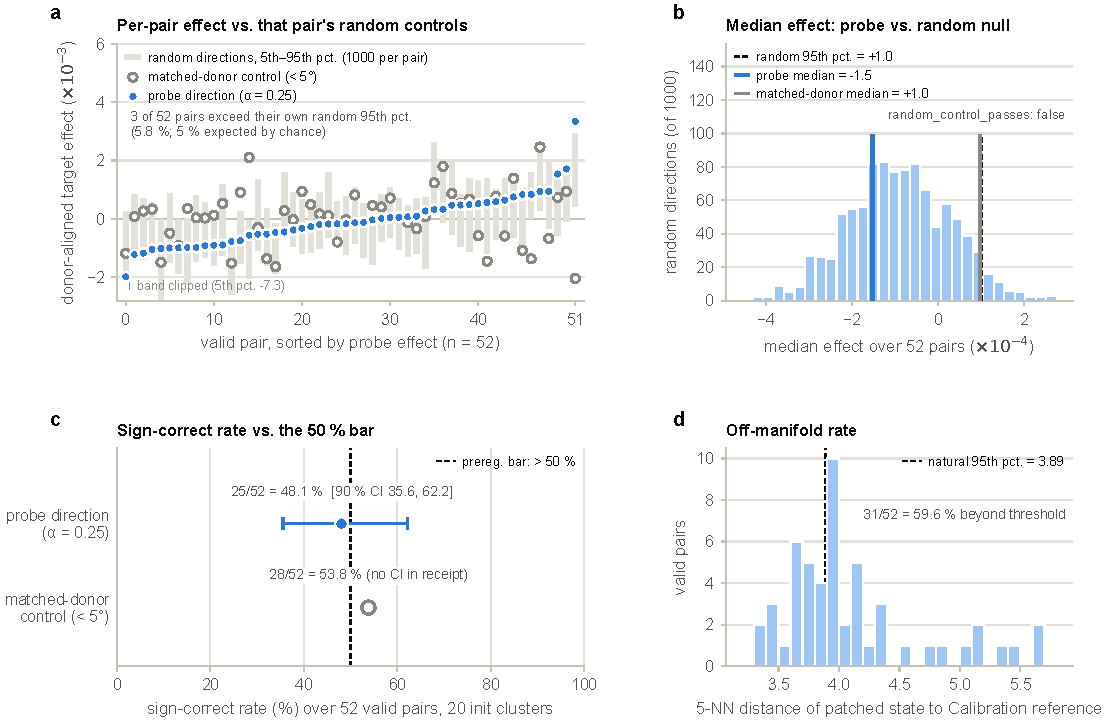
\includegraphics[width=\textwidth]{fig_causal.pdf}
\caption{\textbf{Causal patching at the selected layer (\texttt{early\_expert\_t1\_0}, $\alpha = 0.25$, 52 valid pairs).} \textbf{(a)} Per pair, the donor-aligned effect of the probe direction (blue) against that pair's 5th--95th percentile band over 1\,000 random directions of the same shift norm (grey) and the inert matched-donor control (hollow): 3/52 pairs (5.8\%) exceed their own random 95th percentile, the 5\% expected by chance. \textbf{(b)} The preregistered null: the median-over-pairs effect for each random direction; the probe's median ($-1.5\times10^{-4}$) sits inside the null, below its 95th percentile ($+1.0\times10^{-4}$). \textbf{(c)} Sign-correct rate $25/52 = 48.1\%$ with 90\% cluster interval versus the 50\% bar; matched-donor control $28/52 = 53.8\%$. \textbf{(d)} 5-NN distance of each patched state to the Calibration reference; 31/52 exceed the natural 95th percentile (3.89).}
\label{fig:causal}
\end{figure}

\paragraph{Dose.} Figure~\ref{fig:dose}: at $\alpha = 0.5$ and $1.0$, in every one of the eight conditions, the off-target ratio stays between 1.6 and 8.0 and sign-correct rates scatter from 0\% to 75\% with 4--15 valid pairs per cell---no cell approaches the specificity bar and no dose trend appears (the $\alpha = 0.25$ row, derived from the main evidence, looks the same). Calibration had already shown the same pattern at all three doses (ratios 3.6--5.5), which is why $\alpha$ was frozen at the smallest value rather than tuned upward.

\begin{figure}[htbp]
\centering
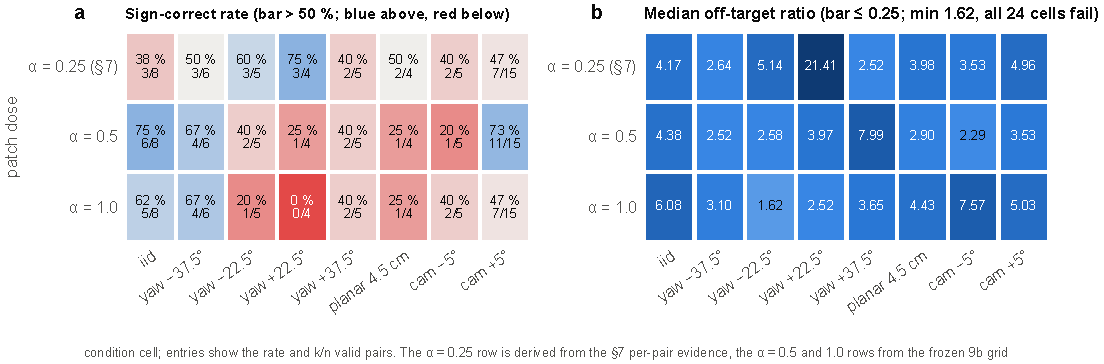
\includegraphics[width=0.9\textwidth]{fig_dose.pdf}
\caption{\textbf{Dose $\times$ condition sensitivity.} \textbf{(a)} Sign-correct rate with valid-pair counts per cell (grey = 50\%, blue above, red below). \textbf{(b)} Median off-target ratio (log scale). Rows $\alpha = 0.5, 1.0$ are the preregistered sensitivity grid; the $\alpha = 0.25$ row is derived from the same pairs in the main causal evidence. Every one of the 24 cells fails the $\leq 0.25$ specificity bar (range 1.6--21.4); sign rates scatter from 0\% to 75\% on 4--15 pairs.}
\label{fig:dose}
\end{figure}

\paragraph{What could not be tested.} The preregistered \emph{confirmatory} mechanistic claim required the direction to agree across at least two of three candidate layers. The frozen probe artifact stores coefficients only for the selected layer; fitting the others after Locked Test access would have been a post-hoc refit, so this criterion is reported as \emph{unavailable} and the confirmatory claim as \emph{unsupported}, exactly as decided before access (Appendix~\ref{app:deviations}). The single-layer evidence above stands on its own.

\paragraph{Interpretation.} The probe direction is decodable because orientation information is present, but the action expert does not read it through this coordinate at this layer---moving it is indistinguishable from noise. Two readings remain open: the used coordinate is elsewhere (different layer, token, or a non-linear function of several directions), or orientation enters the action through the visual pathway in a way that a residual-stream patch at one layer cannot reproduce. Section~\ref{sec:limits} gives our odds.

%======================================================================
\section{Claim 4: no earlier alarm}
\label{sec:claim4}
Thresholds were fixed on Calibration at a 10\% episode-level false-positive rate (\Mz{} 0.541, \Mo{} 0.493, \Mt{} 0.504; alarm = 3 consecutive exceedances at 5-step cadence). On the 60 failed Locked Test episodes, \Mo{} and \Mt{} each detect 59; median lead before the annotated onset is 435 and 422.5 steps respectively, and the \emph{paired} median difference is $0$ with a degenerate interval $[0,0]$: in most failed episodes both alarms fire at the same early step. The large absolute leads reflect that most failures on this task are ``terminal horizon'' failures (on Calibration, 48 of 53) that the state-based models flag almost from the start, not a late, sudden break. Figure~\ref{fig:lead} shows the paired first-alarm steps and the mean probability trajectories.

\begin{figure}[htbp]
\centering
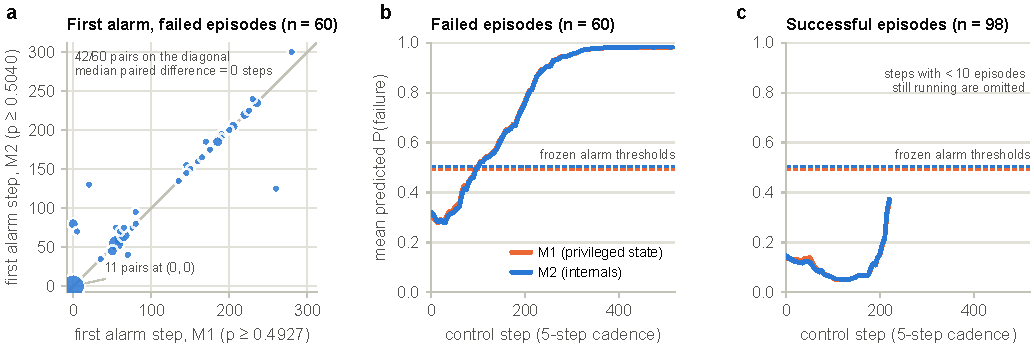
\includegraphics[width=\textwidth]{fig_lead_time.pdf}
\caption{\textbf{Alarms at 10\% episode-FPR.} \textbf{(a)} Paired first-alarm control step of \Mt{} versus \Mo{} on the 60 failed episodes (thresholds \Mo{} 0.493, \Mt{} 0.504); 42/60 pairs lie on the diagonal, marker area $\propto$ coincident pairs; median paired difference 0 steps (bar: $\geq 5$). \textbf{(b, c)} Mean predicted failure probability over control steps for failed ($n{=}60$) and successful ($n{=}98$) episodes; failed episodes cross the thresholds around step 100 on average, and the \Mo{}/\Mt{} curves coincide.}
\label{fig:lead}
\end{figure}

%======================================================================
\section{Limitations and what would change our mind}
\label{sec:limits}
We separate three readings of the negative results and give our rough odds; these are judgments, not measurements.
\begin{itemize}
\item \textbf{Hypothesis false for this policy/task (\Mt{} adds nothing over \Mo{}): $\sim 75\%$.} The interval is tight, the Calibration out-of-fold lift was equally small, and the per-cell pattern is uniform. We would update if a different internal feature set (e.g.\ a probe for gripper--object contact or for the goal compartment) produced a lift $\geq 3\%$ under the same protocol.
\item \textbf{Method insensitive for the causal claim (wrong layer/coordinate, not absence of mechanism): $\sim 40\%$.} The failure is specific: we tested one linear 2-D subspace at one residual location and flow step, with a patch that is smaller than random noise. We would update toward ``mechanism exists'' if patching the VLM-context token or the late expert location, or a non-linear (e.g.\ token-wise) version of the direction, produced a specific, sign-correct effect with the same controls. We would update toward ``no mechanism'' if a probe with much lower MAE at any location still failed specificity.
\item \textbf{Underpowered: $\sim 15\%$ for the prediction claims; $\sim 25\%$ for the causal sign test.} The primary interval excludes the 3\% bar, but a 1--2\% lift would need roughly four times the episodes to resolve. The causal sign interval ($\pm 13$\,pp) could hide a weak true effect, but the specificity failure does not depend on power.
\end{itemize}
Further limits: one policy, one task, 158 episodes; failure labels come from the simulator, not human judgment; the annotated failure \emph{onset} is a deterministic heuristic; the probe is modest (tracks $\sim 15\%$ of a rotation); and the study cannot say anything about SAE-style features or non-linear readouts, which were out of scope by design.

\paragraph{What we would do next, if anything.} Not another run of this design. The informative follow-ups are (i) a cross-layer causal sweep with the same controls, cheap now that the pipeline exists ($\approx$\,3 GPU-hours per layer), and (ii) replacing the orientation probe with a probe for the variable the policy actually fails on (contact/grasp), which the per-cell results suggest.

%======================================================================
\section{Reproducibility and cost}
\label{sec:repro}
Everything is in the repository: preregistration (\texttt{PREREG.md}), every change with date and reason (\texttt{AMENDMENTS.md}), a per-experiment log (\texttt{log.md}), the frozen locks, the runbook, and the final report with all receipts (\texttt{artifacts/locked-test-final-report/}). Every input to the evaluator is content-addressed (Table~\ref{tab:hashes}); the evaluator refuses to run on anything else.

Compute for the Locked Test: collection 4.3 GPU-h (160 rollouts, $\approx 96$\,s each), scoring 14.5 GPU-h (the dominant cost: dozens of forward passes per scored state for the counterfactual transformations and noise draws), causal patching 2.8 GPU-h (60\,120 forward passes), sensitivity 0.1 GPU-h; 21.7 GPU-h and \$14.81 at \$0.68/h on a rented RTX~5090, plus about \$2 of provisioning overhead. The whole month-one study, including Discovery and Calibration, fits in the low tens of GPU-hours.

\begin{table}[htbp]
\centering\small
\caption{Content addresses (SHA-256 prefixes) of the frozen inputs and outputs.}
\label{tab:hashes}
\begin{tabular}{ll}
\toprule
Locked Test manifest & \texttt{1fd8c818} \\
Calibration freeze (probe, predictors, thresholds, $\alpha$) & \texttt{eb39e695} \\
Reality-gate lock & \texttt{4e0d4d5c} \\
Collection receipt (160 artifacts) & \texttt{3314fb71} \\
Frozen predictions & \texttt{86d85ed1} \\
Causal receipt (60 evidence files) & \texttt{5fc67e65} \\
Sensitivity receipt & \texttt{e6dee93e} \\
Cost receipt & \texttt{b2547d51} \\
Final report & \texttt{f7d51bf8} \\
\bottomrule
\end{tabular}
\end{table}

%======================================================================
\appendix
\section{Preregistered decision table and expectation}
\label{app:prereg}
From \texttt{start.md} \S12, fixed on 2 August 2026:
\begin{center}\small
\begin{tabular}{p{0.5\textwidth}p{0.42\textwidth}}
\toprule
Outcome & Consequence \\
\midrule
Lift (\Mt{} $>$ \Mo{}) \textbf{and} specific patching & Month 2: data-acquisition race \\
No average lift, clear advantage on delayed failures & Narrow finding; publish \\
Lift without causal specificity & Good detector, weak mech-interp claim \\
Specificity without lift & Interesting, economically weak; publish \\
\textbf{Neither lift nor specificity} & \textbf{End project, publish negative result} \\
Lift only \Mt{} $>$ \Mz{}, not \Mt{} $>$ \Mo{} & Internals replace privileged state, do not exceed it \\
\bottomrule
\end{tabular}
\end{center}
Pre-stated expectation (\texttt{AMENDMENTS.md}, 25 August, from nine toy experiments): ``\Mt{} approximately \Mo{} with \Mt{} much better than \Mz{}.'' Measured: rows five and six.

\section{Calibration-stage results}
\label{app:calib}
Out-of-fold on Calibration (160 episodes, 107 successes): \Mz{} log loss 0.433 / Brier 0.137 / AUROC 0.828; \Mo{} 0.246 / 0.068 / 0.937; \Mt{} 0.245 / 0.068 / 0.938; \Mt{} vs \Mo{} lift 0.40\% (1.20\% with the coverage features removed), \Mt{} vs \Mz{} 43.4\%. Alpha calibration on 60 Calibration pairs: sign rates 56.7\% / 60.0\% / 51.7\% at $\alpha = 0.25/0.5/1.0$ (all intervals contain 50\%), off-target ratios 4.94 / 3.63 / 5.51, off-manifold 0\%. Probe candidates (circular MAE, rad): VLM context 0.274, early expert $t{=}1.0$ 0.253 (selected), early $t{=}0.5$ 0.248, late $t{=}1.0$ 0.248, late $t{=}0.5$ 0.249; controls: constant 0.332, proprioception-only 0.315, shuffled labels 0.406. Discovery reality gate: 8/10 iid successes, 30/30 valid yaw perturbations, failure rate 0.37 (bar 0.20--0.80).

\section{Locked Test data integrity and per-cell numbers}
\label{app:integrity}
160/160 artifacts with matching provenance (code commit \texttt{18d64941}, policy \texttt{31d453f7}). Two invalid resets (init 47 and 48, cell 5, the 4.5\,cm displacement), a 10\% rate exactly at the preregistered cap; the cell is retained and the two episodes excluded from all estimands. All other validity-envelope rates are zero.
\begin{center}\small
\begin{tabular}{llccc}
\toprule
Cell & Condition & \Mz{} & \Mo{} & \Mt{} \\
& & AUROC / log loss & AUROC / log loss & AUROC / log loss \\
\midrule
0 & iid & 0.504 / 0.716 & 0.694 / 0.667 & 0.712 / 0.663 \\
1 & book yaw $-37.5^\circ$ & 0.713 / 0.537 & 0.780 / 0.416 & 0.763 / 0.438 \\
2 & book yaw $-22.5^\circ$ & 0.566 / 0.492 & 0.696 / 0.439 & 0.706 / 0.437 \\
3 & book yaw $+22.5^\circ$ & 0.725 / 0.635 & 0.933 / 0.487 & 0.951 / 0.456 \\
4 & book yaw $+37.5^\circ$ & 0.801 / 0.590 & 0.976 / 0.210 & 0.980 / 0.204 \\
5 & planar diagonal 4.5\,cm & 0.665 / 0.821 & 0.858 / 0.700 & 0.860 / 0.708 \\
6 & camera yaw $-5^\circ$ & 0.602 / 0.404 & 0.665 / 0.323 & 0.658 / 0.316 \\
7 & camera yaw $+5^\circ$ & 0.514 / 0.921 & 0.732 / 0.934 & 0.729 / 0.935 \\
\bottomrule
\end{tabular}
\end{center}

\section{Deviations and amendments during the Locked Test}
\label{app:deviations}
All recorded prospectively in \texttt{AMENDMENTS.md} before the affected step ran; none touched a scientific quantity.
\begin{itemize}
\item \textbf{Replacement instance.} The original GPU instance had been destroyed by the provider (negative balance) before the Locked Test; the frozen runtime was rebuilt from pinned wheels, source hashes and model snapshots on a new RTX~5090 (\texttt{ops/locked\_test\_bootstrap.sh}); the machine-readable preflight matched the freeze on every field.
\item \textbf{Second scoring worker.} Serial scoring would have exceeded the credit; a second, reverse-walking process was added using the scorer's built-in concurrency (Calibration precedent showed only physical-cost fields differ).
\item \textbf{Two evaluator loader fixes} (trailing newline in the frozen reality-gate lock; read-only mapping type from the artifact loader): each aborted the evaluator at input validation with no output, was unit-tested and committed before the rerun. The successful run was the first to read any outcome.
\item \textbf{Pre-access unavailability decisions} (1 September): the 9a rollout position diagnostic and the supporting-layer coefficients were declared unavailable rather than substituted post hoc; the confirmatory multi-layer claim was therefore fixed as unsupported before the test was opened.
\end{itemize}

\section{How to reproduce}
\label{app:repro}
Clone the repository at tag \texttt{locked-test-score-v1}; follow \texttt{ops/locked\_test\_runbook.md}. The report JSON and every receipt are in \texttt{artifacts/locked-test-final-report/}; the figures in this document are generated by \texttt{make\_figures.py} in that directory from those files alone. The raw rollouts (12\,GB) and score sidecars are mirrored off-instance and available on request.

\end{document}
